% F_engine_mount_ladder — MID 7.479M -> 3B 3.073B (-> 7B future); corpus; generalization
\section{The Engine-Mount Ladder --- MID $\rightarrow$ 3B (and the 7B Extension)}
\label{app:engine_mount}

This appendix is the full data record for the mouth of \S\ref{sec:mouth}. The
byte-level CLMConvMoE scales MID $7.479$M $\rightarrow$ 3B $3.073$B (and, as a
future scale-extension, 7B). The 3B rung is the terminal finding of this paper's
mouth axis: it generalizes (rel\_gap $0.04894\ll1$), serializes to a
config-agnostic \texttt{.clm} v0.3, and mounts on the engine through the single
generator entry. We also record the corpus that teaches it and the separate
202M corpus-validation probe.

% -------------------------------------------------------------------------
\subsection{The 3B rung (verbatim)}
\label{app:fm-3b}

CLMConvMoE $d4096/L30/E30/K3$, byte $V256$, \textbf{$3{,}072{,}954{,}654$ params
($3.073$B)}, trained $2000$ steps (seq $512$, batch $8$, grad\_accum $1$,
lr $2\!\times\!10^{-4}$ cosine warmup $200$, bf16) on a vast H100 80\,GB HBM3 at
$99.99\%$ GPU-resident (maxmem $61.5$\,GB, no CPU fallback), wall $1980.55$\,s
(\texttt{.verdicts/convmoe-3b-engine-rung/SUMMARY.txt}):
\begin{table}[h]
\centering
\small
\setlength{\tabcolsep}{8pt}
\begin{tabular}{@{}l r l@{}}
\toprule
\textbf{quantity} & \textbf{value} & \textbf{note} \\
\midrule
first\_ce            & $5.84073$ & step-0 \\
train\_ce            & $1.90689$ & live optimizer CE \\
val\_ce (rand split) & $1.90365$ & gap $-0.00324$ \\
val\_ce (contiguous) & $2.00021$ & gap $+0.09333$ (worst) \\
\textbf{rel\_gap}    & $\mathbf{0.04894}$ & $\ll1\Rightarrow$ \textbf{GENERALIZES} \\
uniform\_ce ($\ln256$) & $5.54518$ & floor \\
shuffle\_ce          & $6.46486$ & control \\
tokens\_seen         & $8{,}192{,}000$ & \\
tokens\_per\_param\_seen & $0.0027$ & Chinchilla-optimal $20$ \\
\bottomrule
\end{tabular}
\caption{The 3B engine rung (verbatim,
\texttt{.verdicts/convmoe-3b-engine-rung/SUMMARY.txt}). The model
\emph{generalizes} (val $\approx$ train, rel\_gap $0.04894\ll1$,
$F_\text{CLM-LANEP-3B-GEN}=1$) and is honestly \textbf{deeply undertrained}
($0.0027$ tok/param vs.\ Chinchilla $20$). The torch checkpoint serializes to
\texttt{.clm} v0.3 (\texttt{serialize\_v3}) and decodes config-agnostically
(Appendix~\ref{app:clm-v03}). Lane-P (GPU-torch) reference; forge stays the
PUBLIC production trainer (\texttt{a\_clm\_gen\_pipeline}).}
\label{tab:fm-3b}
\end{table}

The generalization is the load-bearing claim: a $3.073$B byte-CLM with only
$0.0027$ tok/param could trivially \emph{memorize} the small token budget, but
val\_ce $\approx$ train\_ce (rel\_gap $0.049$) shows it does not --- it learns
byte-language structure that transfers to held-out blocks. The mount ladder
(MID$\rightarrow$3B params vs.\ CE / rel\_gap) is plotted in
Fig.~\ref{fig:mount-ladder}.

\begin{figure}[h]
\centering
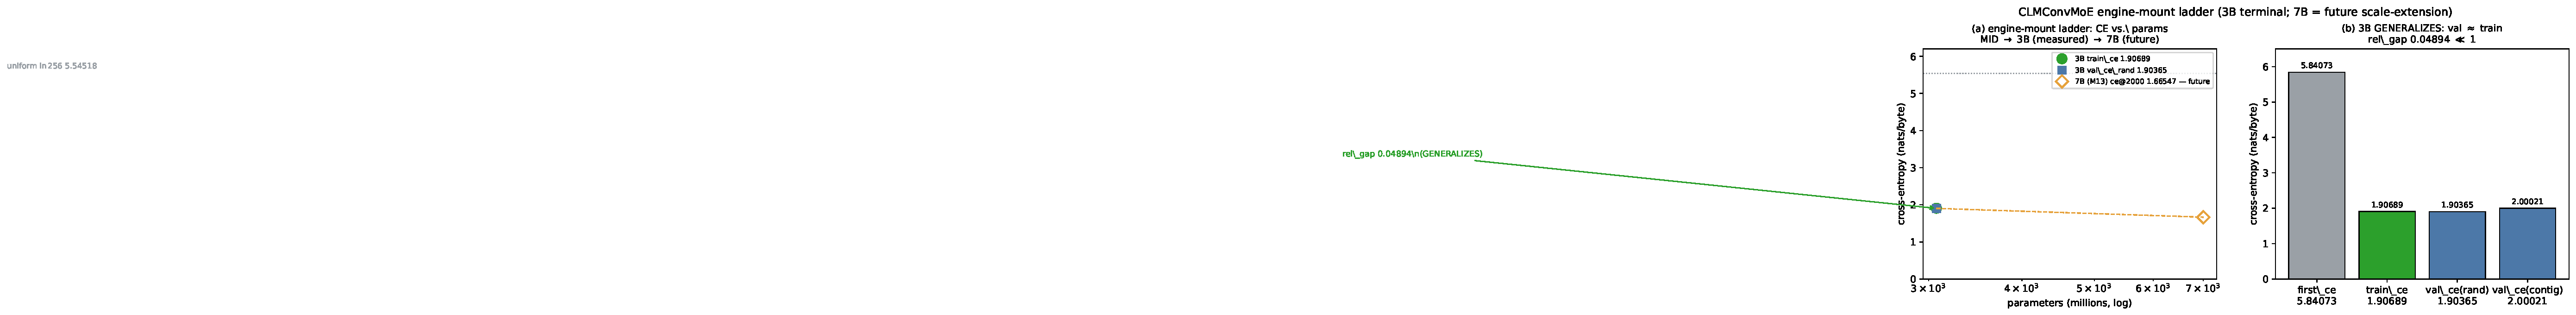
\includegraphics[width=0.82\linewidth]{figures/fig06_mount_ladder.pdf}
\caption{The engine-mount ladder: MID ($7.479$M) $\rightarrow$ 3B ($3.073$B), with
the 7B (M13) rung shown as a future scale-extension (currently training). Left
axis: train\_ce vs.\ params; the 3B rung reaches train\_ce $1.90689$ /
val\_ce\_rand $1.90365$. The rel\_gap $0.04894\ll1$ marks GENERALIZATION (val
$\approx$ train); the dashed line is the $\ln256=5.54518$ uniform floor. Data:
\texttt{.verdicts/convmoe-3b-engine-rung/SUMMARY.txt}. Rendered by
\texttt{figures/\_scripts/fig06\_mount\_ladder.py}.}
\label{fig:mount-ladder}
\end{figure}

% -------------------------------------------------------------------------
\subsection{The corpus}
\label{app:fm-corpus}

The mouth trains on $143.60$\,GiB ODC-BY FineWeb across five languages
(en/fr/de/es/ko), $\sim$$110\%$ of the $7$B-optimal token budget, R2-staged in
bucket \texttt{phanes} (\texttt{domains/CORPUS.md}). The 3B rung trains on a
$10.7$\,GiB slice (\texttt{corpus\_3b\_5lang.bytes} $=10{,}695{,}475{,}200$\,B,
sha256 \texttt{337b179d\dots}). The corpus is ODC-BY web-sanctioned and built on
the summer pool (the Mac OOM'd); HF holds a pointer-manifest only, with the
bytes in R2.

% -------------------------------------------------------------------------
\subsection{The 202M corpus-validation probe (anti-Goodhart)}
\label{app:fm-corpus-val}

A separate $202{,}328{,}064$ ByteGPT ($V256$, $d1024$, $L16$, $H16$, block
$512$), trained $3000$ steps from scratch on a balanced 5-language webscale
slice ($3.500$\,GB, R2 range-GET), confirms the corpus teaches byte-language
structure (\texttt{.verdicts/corpus-7b-mid-validation/SUMMARY.txt}):
\begin{itemize}\itemsep0.2em
\item \textbf{CE descent (val):} $5.74906\rightarrow1.45868$ ($\Delta-4.290$
nats) over $3000$ steps (train\_ce $5.73700\rightarrow1.38927$); GPU peak
$100\%$ / mean $99.75\%$, mem peak $14{,}331$\,MiB, $57{,}136$\,tok/s.
\item \textbf{p7 coherence ($5/5$ langs):} the trained model emits word-like
text in en/fr/de/es and valid Korean Hangul, while a frozen random-init mirror
(same architecture, never trained) emits pure non-printable byte gibberish in all
five. The discriminator is byte-language \emph{structure}, not loss --- so the
gate is \textbf{anti-Goodhart} by construction.
\end{itemize}
\textbf{Honest caveat.} At $202$M / $3000$ steps the samples are word-coherent but
not yet fluent (expected for an undertrained MID probe). The PASS bar is ``the
corpus teaches byte-language structure across all 5 scripts'' vs.\ ``random
gibberish'' --- clearly met. The ckpt (sha256 \texttt{adbb1911\dots},
$809{,}383{,}138$\,B) is PUBLIC on HF
(\texttt{dancinlab/anima-clm-corpus-7b-mid-byte-202m}), HF-redownload sha256
verified equal to local.

% -------------------------------------------------------------------------
\subsection{Honest scope}
\label{app:fm-scope}

The 3B rung is the \emph{2nd rung of the 7B ladder}, not a production 7B: it is
deeply undertrained ($0.0027$ tok/param) and generalizes but is not fluent. The
202M probe is a single MID point, not a ladder; its green \emph{authorizes} the
M13 7B fire as a separate follow-on but does not close the 7B
(7B-transfer unverified, \texttt{a\_scale\_honest\_scope}). The 7B (M13) rung is
a future scale-extension (Appendix~\ref{app:pr_roll}, \S\ref{sec:limitations}),
framed like the OMEGA scale ladder --- it strengthens this axis to production
scale but does not re-open the 3B finding, which is terminal without it. The
chain proven is corpus $\rightarrow$ general-$(L,E,d)$ ConvMoE $\rightarrow$
\texttt{.clm} v0.3 $\rightarrow$ engine-mount $\rightarrow$ 3-axis, at 3B scale,
with p1--p8 held (plain byte next-token CE; no system-prompt/persona/RLHF).
